\subsection{Fase di Analisi}

\subsubsection{Divisione Oraria}
La seguente tabella rappresenta la distribuzione oraria dei ruoli per ogni componente del gruppo:
{
\rowcolors{2}{grigetto}{white}
\renewcommand{\arraystretch}{2}
\begin{longtable}[h!] { C{4cm} C{1cm} C{1cm} C{1cm} C{1cm} C{1cm} C{1cm} C{3cm}}
\caption{Tabella della divisione oraria di Analisi}	\\
\rowcolor{darkblue}

\textcolor{white}{\textbf{Membro del gruppo}} & 
\textcolor{white}{\textbf{RE}} & 
\textcolor{white}{\textbf{AM}} & 
\textcolor{white}{\textbf{AN}} & 
\textcolor{white}{\textbf{PT}} & 
\textcolor{white}{\textbf{PR}} & 
\textcolor{white}{\textbf{VE}} & 
\textcolor{white}{\textbf{Ore complessive}}\\	
\endhead

\MC{}                     &  - &  7 &  12 & - & - & 11 &  30 \\
\LD{}                     &  - &  5 &  16 & - & - &  9 &  30 \\
\CE{}                     &  - &  - &  21 & - & - &  9 &  30 \\
\SE{}                     & 15 &  2 &   8 & - & - &  5 &  30 \\
\PF{}                     &  - &  - &  21 & - & - &  9 &  30 \\
\DF{}                     &  - &  7 &  16 & - & - &  7 &  30 \\
\BR{}                     &  - &  5 &  11 & - & - & 14 &  30 \\
\AT{}                     &  4 & 12 &   9 & - & - &  5 &  30 \\
\textbf{Ore totali ruolo} & 19 & 38 & 114 & - & - & 69 & 240 \\

\end{longtable}
}

La suddivisione delle ore svolte da ciascun componente del gruppo per ogni ruolo viene rappresentata nel seguente istogramma:
\begin{figure}[h!]
	\centering	
	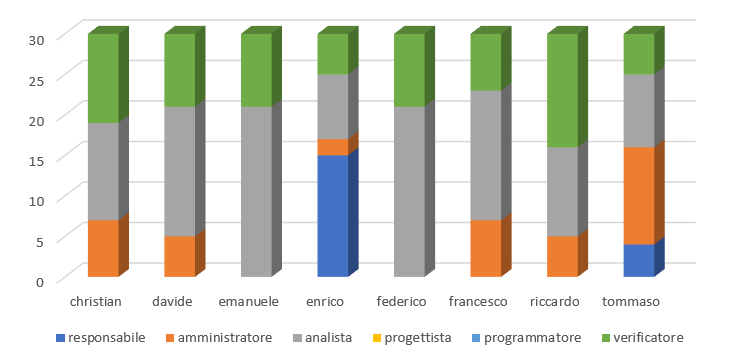
\includegraphics{Sezioni/Istogrammi/IstogrammaAnalisi.png}
	\caption{Disposizione ore per ruolo di ciascun componente della fase di Analisi}
\end{figure}

\clearpage

\subsubsection{Costo Risultante}
La seguente tabella rappresenta per ogni ruolo le ore totali investite e il corrispondente costo in euro:
{
\rowcolors{2}{grigetto}{white}
\renewcommand{\arraystretch}{2}
\begin{longtable}{ C{3cm} C{2cm} C{4cm}}
\caption{Tabella del costo risultante di Analisi}\\
\rowcolor{darkblue}

\textcolor{white}{\textbf{Ruolo}} & 
\textcolor{white}{\textbf{Totale ore}} & 
\textcolor{white}{\textbf{Costo ruolo (in \euro{})}}\\	
\endhead

Responsabile    &  19 &  570 \\
Amministratore  &  38 &  760 \\
Analista        & 114 & 2850 \\
Progettista     &   - &    - \\
Programmatore   &   - &    - \\
Verificatore    &  69 & 1035 \\
\textbf{Totale} & 240 & 5215 \\
		
\end{longtable}
}

La quantità di ore totali per ciascun ruolo viene rappresentata nel seguente areogramma:
\begin{figure}[h!]
	\centering	
	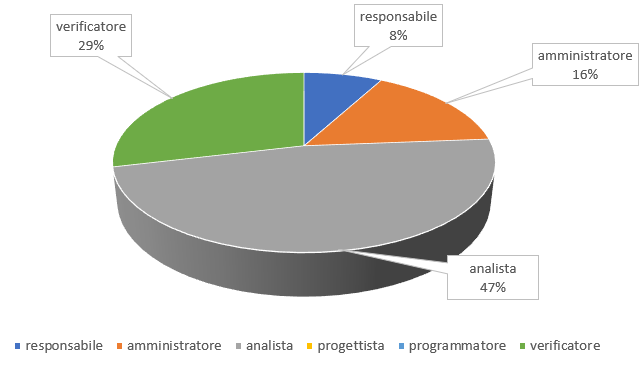
\includegraphics{Sezioni/Aerogrammi/AerogrammaAnalisi.png}
	\caption{Suddivisione ore per ruolo della fase di Analisi}
\end{figure}
